\documentclass[12pt,a4paper,oneside]{report}

% =========================================================================
% TIET REPORT FORMAT GUIDELINES CONFIGURATION
% 1. Type: Single Side, Colored
% 2. Paper Size: A4 (portrait)
% 3. Margins: 1.5 in Left (Binding), 1.0 in Top / Bottom / Right
% 4. Font Type: Times New Roman (mathptmx)
% 5. Font Sizes: 16pt bold (Chapters), 14pt bold (Sections), 12pt (Body)
% 6. Line Spacing: 1.5 throughout
% 7. Page Numbering: Bottom center (Roman for Prelims, Arabic for Chapters)
% 8. Table Content Font: 10pt (\small)
% 9. Captions Font: 10pt Bold
% 10. References: Single-spaced, justified, IEEE square bracket citations
% =========================================================================

\usepackage[left=1.5in, right=1.0in, top=1.0in, bottom=1.0in]{geometry}
\usepackage{mathptmx} % Times New Roman
\usepackage[T1]{fontenc}
\usepackage[utf8]{inputenc}
\usepackage{setspace}
\setstretch{1.5} % 1.5 line spacing throughout

\usepackage{titlesec}
\usepackage{fancyhdr}
\usepackage{graphicx}
\usepackage{booktabs}
\usepackage{tabularx}
\usepackage{array}
\usepackage{multirow}
\usepackage{makecell}
\usepackage[table]{xcolor}
\usepackage{listings}
\usepackage{amsmath, amssymb}
\usepackage{float}
\usepackage{enumitem}
\usepackage{microtype}
\usepackage{tocloft}
\usepackage[hidelinks]{hyperref}

% -------------------------------------------------------------------------
% COLOR DEFINITIONS
% -------------------------------------------------------------------------
\definecolor{SlateDark}{HTML}{0F172A}
\definecolor{SlateMuted}{HTML}{475569}
\definecolor{NavyBlue}{HTML}{1E3A8A}
\definecolor{RoyalBlue}{HTML}{2563EB}
\definecolor{DarkGreen}{HTML}{14532D}
\definecolor{BorderGray}{HTML}{CBD5E1}
\definecolor{HeaderGray}{HTML}{F1F5F9}
\definecolor{AccentGreen}{HTML}{F0FDF4}

% -------------------------------------------------------------------------
% CAPTION & HEADING STYLES PER GUIDELINES
% -------------------------------------------------------------------------
\usepackage[font={small,bf},labelfont=bf,labelsep=colon]{caption}

% Chapter headings: 16pt Bold
\titleformat{\chapter}[block]
  {\fontsize{16pt}{20pt}\selectfont\bfseries\color{SlateDark}}
  {\thechapter. }
  {0pt}
  {}
\titlespacing*{\chapter}{0pt}{-18pt}{12pt}

% Section headings: 14pt Bold
\titleformat{\section}
  {\fontsize{14pt}{18pt}\selectfont\bfseries\color{SlateDark}}
  {\thesection}
  {1em}
  {}
\titlespacing*{\section}{0pt}{12pt}{5pt}

% Subsection headings: 13pt Bold
\titleformat{\subsection}
  {\fontsize{13pt}{17pt}\selectfont\bfseries\color{SlateDark}}
  {\thesubsection}
  {1em}
  {}
\titlespacing*{\subsection}{0pt}{9pt}{3pt}

% Paragraph settings: Justified with 0.3in first line indent
\setlength{\parindent}{0.3in}
\setlength{\parskip}{0pt}

% Page numbering: Bottom Center
\pagestyle{fancy}
\fancyhf{}
\fancyfoot[C]{\thepage}
\renewcommand{\headrulewidth}{0pt}
\renewcommand{\footrulewidth}{0pt}

% Compact TOC formatting to fit strictly on 2 pages
\setlength{\cftbeforechapskip}{3pt}
\setlength{\cftbeforesecskip}{1pt}
\setlength{\cftbeforesubsecskip}{0pt}
\renewcommand{\cftchapleader}{\cftdotfill{\cftdotsep}}
\renewcommand{\cftsecleader}{\cftdotfill{\cftdotsep}}
\renewcommand{\cftsubsecleader}{\cftdotfill{\cftdotsep}}

% List customization
\setlist[itemize]{leftmargin=0.35in, itemsep=1.5pt, topsep=1.5pt, parsep=0pt}
\setlist[enumerate]{leftmargin=0.35in, itemsep=1.5pt, topsep=1.5pt, parsep=0pt}

% Code snippet styling
\lstset{
  basicstyle=\fontsize{9pt}{12pt}\selectfont\ttfamily,
  backgroundcolor=\color{HeaderGray},
  frame=single,
  rulecolor=\color{BorderGray},
  breaklines=true,
  keywordstyle=\color{RoyalBlue}\bfseries,
  commentstyle=\color{SlateMuted}\itshape,
  stringstyle=\color{DarkGreen},
  keepspaces=true,
  showstringspaces=false
}

\begin{document}

% =========================================================================
% 1. COVER PAGE / TITLE PAGE (No Page Number)
% =========================================================================
\begin{titlepage}
\centering
\thispagestyle{empty}

\vspace*{0.1in}
{\fontsize{18pt}{22pt}\selectfont\bfseries\color{SlateDark} HONEY-LLM: AN INTERACTIVE, SELF-HEALING HONEYPOT DEFENSE ECOSYSTEM FOR AGENTIC AI \par}

\vspace{0.2in}
{\fontsize{13pt}{17pt}\selectfont\bfseries Capstone Project Report \par}
\vspace{0.04in}
{\fontsize{12pt}{16pt}\selectfont\bfseries MID SEMESTER EVALUATION (Phases 1 to 4 Progress) \par}

\vspace{0.25in}
{\fontsize{12pt}{16pt}\selectfont\bfseries Submitted by: \par}
\vspace{0.08in}
{\fontsize{12pt}{16pt}\selectfont
\textbf{(102303312) ANOUSHKA SINGH} \\
\textbf{(102303315) TARUN KRISHNA SHASTRI} \\
\textbf{(102303631) DEVANSH WADHWANI} \\
\textbf{(102303684) SHREYA GIRI} \par}

\vspace{0.18in}
{\fontsize{12pt}{16pt}\selectfont
BE Third Year, Computer Engineering (CoE) \\
\textbf{CPG No: 75} \par}

\vspace{0.2in}
{\fontsize{12pt}{16pt}\selectfont Under the Mentorship of: \par}
\vspace{0.04in}
{\fontsize{12pt}{16pt}\selectfont\textbf{Dr. Saif Nalband} \\
Assistant Professor, Computer Science and Engineering Department \par}

\vspace{0.25in}

\includegraphics[width=1.5in]{assets/thapar_logo.png}

\vspace{0.2in}
{\fontsize{12pt}{16pt}\selectfont\bfseries
Computer Science and Engineering Department \\
Thapar Institute of Engineering and Technology, Patiala \\
August 2026 \par}

\end{titlepage}

% =========================================================================
% PRELIMINARY PAGES (Roman Numerals i to viii)
% =========================================================================
\pagenumbering{roman}
\setcounter{page}{1}

% -------------------------------------------------------------------------
% ABSTRACT (Page i) - strictly fits on 1 page
% -------------------------------------------------------------------------
\chapter*{ABSTRACT}
\addcontentsline{toc}{chapter}{ABSTRACT}
\hrule height 1.2pt
\vspace{0.12in}

\begin{spacing}{1.28}
As generative Artificial Intelligence and Large Language Models (LLMs) transition from exploratory conversational tools to autonomous enterprise agents executing multi-turn workflows, they introduce critical security vulnerabilities. Chief among these is adversarial prompt injection, where attackers manipulate natural-language instructions to bypass safety guardrails, hijack system roles, and exfiltrate proprietary corporate assets. Conventional perimeter defenses, including static Web Application Firewalls (WAFs) and rigid keyword matchers, operate on a reactive rejection paradigm that inadvertently reveals filter boundaries to attackers while failing against multi-turn semantic chaining.

This capstone project presents the design, system architecture, and verified implementation of \textbf{Honey-LLM}, covering work completed across \textbf{Phases 1 through 4} of the academic project roadmap. Specifically, the mid-semester implementation achieves four core deliverables: (1) an 8-class Adversarial Threat Taxonomy tailored to conversational enterprise agents; (2) a multi-tier \textit{Intent Sieve} combining a $\sim$2.1 ms P50 benign fast-path statistical classifier (Tier-1) with an authoritative 8B moderation model governed by a custom prompt injection policy (Llama-Guard 3~\cite{llamaguard3}), achieving a \textbf{95.8\% adversarial recall on JailbreakBench~\cite{jailbreakbench2024}} and \textbf{98.3\% adversarial detection recall across the combined 889-sample evaluation corpus} (559/569 adversarial payloads intercepted, 98.9\% overall classification accuracy) while maintaining a \textbf{0.0\% False Positive Rate} on the benign domain evaluation split (0/320 legitimate customer queries flagged); (3) a containerized zero-trust deception sandbox termed the \textit{Mirror Maze} running an LLM-driven decoy persona that dynamic-hallucinates synthetic bait to absorb attacker reconnaissance (verified with \textbf{no container escapes observed across 5/5 executed penetration probes}); and (4) an \textit{Autonomous Guardrail Synthesis} feedback loop that distills captured exploit patterns into formal \textbf{NVIDIA NeMo Colang} rules~\cite{nemo2024guardrails}, hot-patching live gateway policies in \textbf{10.4 seconds} with zero service interruption. The subsequent project lifecycle, comprising Phase 5 (SOC Threat Intelligence Dashboard) and Phase 6 (Empirical Red-Teaming via Microsoft PyRIT~\cite{pyrit2024}), forms the roadmap for the final semester submission.

\vspace{0.08in}
\noindent\textbf{Keywords:} Generative AI Security, Prompt Injection, Semantic Intent Sieve, LLM Honeypot, Autonomous Guardrails, NVIDIA NeMo, Zero-Trust Containerization.
\end{spacing}

\newpage

% -------------------------------------------------------------------------
% DECLARATION (Page ii)
% -------------------------------------------------------------------------
\chapter*{DECLARATION}
\addcontentsline{toc}{chapter}{DECLARATION}
\hrule height 1.2pt
\vspace{0.15in}

We hereby declare that the design principles, experimental methodologies, system implementation, and working prototype model of the capstone project entitled \textbf{``HONEY-LLM: AN INTERACTIVE, SELF-HEALING HONEYPOT DEFENSE ECOSYSTEM FOR AGENTIC AI''} is an authentic record of our own work completed up to \textbf{Phase 4 (Autonomous Guardrail Synthesis and Policy Hardening)} in the Computer Science and Engineering Department, Thapar Institute of Engineering and Technology (TIET), Patiala, under the mentorship and guidance of \textbf{Dr. Saif Nalband} during the academic semester (August 2026).

We further confirm that this report has not been submitted in part or full to any other University or Institution for the award of any degree or diploma.

\vspace{0.15in}
\noindent\textbf{Date:} August 20, 2026

\vspace{0.15in}
\noindent
\small
\begin{tabularx}{\textwidth}{@{}p{1.3in} p{2.2in} X@{}}
\rowcolor{HeaderGray} \textbf{Roll No.} & \textbf{Name of Student} & \textbf{Signature} \\
\hline
102303312 & Anoushka Singh & \rule{1.5in}{0.4pt} \\
102303315 & Tarun Krishna Shastri & \rule{1.5in}{0.4pt} \\
102303631 & Devansh Wadhwani & \rule{1.5in}{0.4pt} \\
102303684 & Shreya Giri & \rule{1.5in}{0.4pt} \\
\hline
\end{tabularx}

\vspace{0.3in}
\noindent\textbf{Counter Signed By:}

\vspace{0.1in}
\noindent
\begin{minipage}{0.5\textwidth}
\textbf{Faculty Mentor:} \\[0.05in]

\includegraphics[width=1.0in]{assets/saif_nalband_signature.jpg} \\[0.05in]
\textbf{Dr. Saif Nalband} \\
Assistant Professor, CSED \\
TIET, Patiala
\end{minipage}

\newpage

% -------------------------------------------------------------------------
% ACKNOWLEDGEMENT (Page iii)
% -------------------------------------------------------------------------
\chapter*{ACKNOWLEDGEMENT}
\addcontentsline{toc}{chapter}{ACKNOWLEDGEMENT}
\hrule height 1.2pt
\vspace{0.15in}

We would like to express our deepest gratitude and heartfelt thanks to our respected project mentor, \textbf{Dr. Saif Nalband}, Assistant Professor, Computer Science and Engineering Department, Thapar Institute of Engineering and Technology, Patiala. His profound domain expertise, constructive technical criticism, constant encouragement, and intellectual guidance throughout the formulation and implementation of the initial four phases of Honey-LLM have been indispensable in steering this research to a successful milestone.

We extend our sincere thanks to \textbf{Dr. Neeraj Kumar}, Professor and Head of the Computer Science and Engineering Department, for providing state-of-the-art laboratory infrastructure, computational facilities, and an academic environment conducive to advanced systems research.

We also acknowledge the collective support of the faculty and technical staff of the Computer Science and Engineering Department at TIET, whose valuable academic perspectives helped refine our software architecture and evaluation methodologies. Furthermore, we are deeply grateful to our peers who supported adversarial dataset curation.

Lastly, we express our profound gratitude to our families and parents for their unyielding patience, emotional encouragement, and steadfast moral support throughout our academic journey.

\vspace{0.25in}
\noindent\textbf{Project Team Members:} \\
Anoushka Singh (102303312), Tarun Krishna Shastri (102303315), \\
Devansh Wadhwani (102303631), Shreya Giri (102303684)

\newpage

% -------------------------------------------------------------------------
% TABLE OF CONTENTS (Pages iv & v)
% -------------------------------------------------------------------------
\begin{spacing}{1.18}
\tableofcontents
\end{spacing}
\newpage

% -------------------------------------------------------------------------
% LIST OF TABLES (Page vi)
% -------------------------------------------------------------------------
\begin{spacing}{1.2}
\listoftables
\addcontentsline{toc}{chapter}{LIST OF TABLES}
\end{spacing}
\newpage

% -------------------------------------------------------------------------
% LIST OF FIGURES (Page vii)
% -------------------------------------------------------------------------
\begin{spacing}{1.2}
\listoffigures
\addcontentsline{toc}{chapter}{LIST OF FIGURES}
\end{spacing}
\newpage

% -------------------------------------------------------------------------
% LIST OF ABBREVIATIONS (Page viii) - direct non-floating table
% -------------------------------------------------------------------------
\chapter*{LIST OF ABBREVIATIONS}
\addcontentsline{toc}{chapter}{LIST OF ABBREVIATIONS}
\hrule height 1.2pt
\vspace{0.12in}

\begin{spacing}{1.1}
\noindent
\small
\begin{tabularx}{\textwidth}{@{}p{1.2in} X@{}}
\rowcolor{HeaderGray} \textbf{Abbreviation} & \textbf{Full Expansion} \\
\hline
\textbf{AI} & Artificial Intelligence \\
\textbf{API} & Application Programming Interface \\
\textbf{CGRP} & Control Group (Linux Resource Control Subsystem) \\
\textbf{CPG} & Capstone Project Group \\
\textbf{DAN} & Do Anything Now (Adversarial Jailbreak Archetype) \\
\textbf{DoS} & Denial of Service \\
\textbf{FASTAPI} & High-Performance Asynchronous Python Web Framework \\
\textbf{FPR} & False Positive Rate \\
\textbf{GPU} & Graphics Processing Unit \\
\textbf{HTTP} & Hypertext Transfer Protocol \\
\textbf{IP} & Internet Protocol \\
\textbf{JSON} & JavaScript Object Notation \\
\textbf{LLM} & Large Language Model \\
\textbf{LOF} & List of Figures \\
\textbf{LOT} & List of Tables \\
\textbf{LR} & Logistic Regression \\
\textbf{NeMo} & Neural Modules Guardrails Framework (NVIDIA) \\
\textbf{OWASP} & Open Web Application Security Project \\
\textbf{PyRIT} & Python Risk Identification Tool for Generative AI \\
\textbf{RAG} & Retrieval-Augmented Generation \\
\textbf{REST} & Representational State Transfer \\
\textbf{SLM} & Small Language Model \\
\textbf{SOC} & Security Operations Center \\
\textbf{SRS} & Software Requirement Specification \\
\textbf{SSE} & Server-Sent Events \\
\textbf{TF-IDF} & Term Frequency -- Inverse Document Frequency \\
\textbf{TIET} & Thapar Institute of Engineering and Technology \\
\textbf{TOC} & Table of Contents \\
\textbf{UID} & User Identifier (POSIX System Security) \\
\textbf{UML} & Unified Modeling Language \\
\textbf{VRAM} & Video Random Access Memory \\
\textbf{WAF} & Web Application Firewall \\
\hline
\end{tabularx}
\end{spacing}

\newpage

% =========================================================================
% MAIN REPORT BODY (Arabic Numerals 1 to 23)
% =========================================================================
\pagenumbering{arabic}
\setcounter{page}{1}

% =========================================================================
% CHAPTER 1: INTRODUCTION
% =========================================================================
\chapter{INTRODUCTION}

\section{Project Overview}
In the contemporary enterprise computing landscape of 2026, Large Language Models (LLMs) have evolved beyond isolated text generation interfaces into deeply integrated autonomous agents. Modern enterprise deployments rely on LLMs to automate mission-critical customer operations, query private structured databases, orchestrate multi-step API workflows, and execute tool-use tasks~\cite{openai2023gpt4}. However, this rapid operational adoption has outpaced conventional cybersecurity paradigms, exposing a profound vulnerability surface known as the semantic attack vector~\cite{owasp2023top10}.

Unlike traditional software systems where security boundaries are strictly demarcated between binary executable code and passive data buffers, LLMs process system instructions, operational context, and untrusted user inputs within a single unified semantic channel. Consequently, malicious actors exploit this architectural reality through Adversarial Prompt Injection and Jailbreaking techniques~\cite{owasp2023top10}. Attackers craft persuasive, contextually masked natural-language payloads, ranging from direct role overrides to indirect prompt injections embedded in retrieved enterprise documents, to manipulate the underlying model into bypassing access controls.

Traditional perimeter defenses, such as Web Application Firewalls (WAFs), heuristic keyword matchers, and static regular expressions, are fundamentally inadequate against semantic attacks. They lack linguistic context, cannot track conversational state across multi-turn sessions, and are trivially bypassed through character obfuscation or subtle adversarial paraphrasing. More critically, standard security mechanisms follow a rigid block-and-alert model. When a malicious query is blocked with an explicit refusal message, the attacker immediately learns the perimeter filtering boundary and iterates their attack prompt until an evasion succeeds.

To systematically address these defensive limitations, this capstone project develops and demonstrates \textbf{Honey-LLM}: an interactive, self-hardening defense ecosystem for conversational AI architectures. For the Mid-Semester Evaluation, the project team has fully developed, integrated, and verified the first four engineering phases:
\begin{itemize}
    \item \textbf{Phase 1 (Adversarial Profiling \& Threat Taxonomy):} Formulated an 8-class threat taxonomy mapping prompt injections to specific enterprise manifestations and validated concurrent dual-model local inference.
    \item \textbf{Phase 2 (The Multi-Tier Semantic Intent Sieve):} Constructed an intelligent input-filtering pipeline that inspects queries in real time, pairing a $\sim$2.1 ms P50 benign fast-path statistical classifier (Tier-1) with an authoritative 8B moderation model governed by a custom prompt injection policy (Llama-Guard 3~\cite{llamaguard3}), achieving a 95.8\% adversarial recall on JailbreakBench~\cite{jailbreakbench2024} and 98.3\% adversarial detection recall across 889 evaluation prompts (559/569 adversarial payloads intercepted, 98.9\% overall accuracy) at a 0.0\% False Positive Rate on benign domain traffic (0/320 benign queries flagged).
    \item \textbf{Phase 3 (The `Mirror Maze' Deception Honeypot):} Deployed an isolated zero-trust Docker sandbox hosting the `Sarah' decoy persona, which dynamic-hallucinates synthetic bait to absorb attacker reconnaissance without leaking real infrastructure.
    \item \textbf{Phase 4 (Autonomous Guardrail Synthesis):} Implemented a closed self-healing loop that distills captured exploits into validated NVIDIA NeMo Colang rules~\cite{nemo2024guardrails}, hot-patching live gateway policies in 10.4 seconds with zero downtime.
\end{itemize}

\section{Need Analysis}
\subsection{The `Smart Mirror' Trap: Enterprise Adoption vs. Defensive Lag}
Industry surveys indicate that enterprise adoption of conversational AI agents has expanded rapidly across customer-facing workflows~\cite{openai2023gpt4}. However, defensive capabilities have lagged behind offensive prompt exploitation techniques. Conventional static honeypots are quickly identified and abandoned by automated scanners. In contrast, generative honeypots offer dynamic semantic interaction, creating an essential observation window to capture zero-day exploitation techniques before they reach production services.

\subsection{The Shift: Machine-Speed Autonomous Warfare}
With conversational models managing automated customer dialogues~\cite{openai2023gpt4}, adversarial techniques have shifted from manual, one-off jailbreaks to automated, machine-speed offensive frameworks (such as ARACNE, Garak, and Microsoft PyRIT~\cite{pyrit2024}). Automated offensive agents can systematically discover exploitable prompt sequences across iterative conversational turns, compressing vulnerability discovery timelines and rendering human-reliant triage workflows ineffective.

\subsection{The `Shadow Trust' Gap: Vulnerability of the Semantic Layer}
Prompt injection is categorized as the primary vulnerability in the OWASP Top 10 for Large Language Model Applications (LLM01)~\cite{owasp2023top10}. Because conversational agents are granted operational trust to execute database lookups and internal APIs, a compromised prompt inherits the agent's broad permissions. In multi-turn dialogue, gradual semantic drift and contextual grooming can frequently bypass static refusal boundaries in unprotected commercial systems.

\subsection{The Dynamic Security Window: Addressing Reactive Lag}
Standard commercial defense workflows require human security analysts to triage incident logs, manually construct mitigation patches, and redeploy models over multi-week cycles. Honey-LLM eliminates this operational lag by autonomously converting captured honeypot interaction transcripts into formal guardrail rules in memory, closing the vulnerability window within seconds of an attempted compromise.

\section{Research Gaps}
A critical review of generative AI defense literature reveals five central research gaps:
\begin{enumerate}
    \item \textbf{Absence of Real-Time Intent Filtering Prior to Sandbox Interaction:} Existing LLM honeypots route all incoming traffic directly into expensive generative sandboxes, degrading benign response throughput and incurring substantial compute overhead.
    \item \textbf{Vulnerability of LLM Decoys to Accidental Ground-Truth Leakage:} Unconstrained generative sandboxes frequently leak authentic corporate architecture or hallucinate uncoordinated internal data during adversarial prompt exploitation.
    \item \textbf{Lack of Autonomous Feedback Loops (Zero-Downtime Policy Hardening):} Current honeypot architectures passively store forensic interaction logs without automating defensive rule generation, requiring manual intervention to update gateway filters.
    \item \textbf{Inadequate Isolation Guarantees in Generative Sandboxes:} Most generative honeypot prototypes execute without strict kernel-level namespace sandboxing, exposing host environments to code execution and egress network scanning vulnerabilities.
    \item \textbf{Latency Overhead of Large Moderation Models:} High-parameter moderation networks introduce unacceptable 700--1500 ms delays into real-time conversational user experiences when applied uniformly to all incoming traffic.
\end{enumerate}

\section{Problem Definition and Scope}
To architect, implement, and empirically validate an automated, dual-tier cybersecurity defense ecosystem for enterprise conversational AI that intercepts adversarial prompt injection payloads, isolates attackers within a containerized generative deception sandbox, and synthesizes permanent, hot-patchable guardrail policies with zero service disruption.

\noindent\textbf{Scope of Mid-Semester Evaluation (Phases 1 to 4):}
\begin{itemize}
    \item Formulation and dataset curation of an 8-Class Adversarial Threat Taxonomy (S1--S8).
    \item Development and threshold calibration of the Multi-Tier Semantic Intent Sieve ($P_{\text{benign}} < 0.15$).
    \item Implementation of the isolated Docker-based `Mirror Maze' deception sandbox on port \texttt{:9100} with zero-egress policies.
    \item Engineering of the closed-loop Autonomous Guardrail Synthesis pipeline compiling NVIDIA NeMo Colang 2.0 rules [6].
    \item Empirical validation of classification accuracy, benign false-positive rates, container isolation, and time-to-patch latency.
\end{itemize}

\section{Assumptions and Constraints}
\begin{table}[H]
\small
\renewcommand{\arraystretch}{1.2}
\caption{System Assumptions and Engineering Constraints}
\begin{tabularx}{\textwidth}{@{}p{1.4in} X@{}}
\rowcolor{HeaderGray} \textbf{Category} & \textbf{Operational Specification \& Constraint} \\
\hline
\textbf{Hardware Constraint} & Single enterprise host with $\ge$16 GB unified RAM / VRAM, supporting simultaneous execution of dual 8B parameter models. \\
\textbf{Model Assumption} & Base enterprise agents utilize Llama-3 8B Instruct; secondary moderation utilizes Llama-Guard 3 8B. \\
\textbf{Isolation Constraint} & Zero-egress network policies on Docker sandbox; non-root execution (UID 10001); read-only root filesystems. \\
\textbf{Language Constraint} & Current dataset coverage focuses on English-language conversational dialogues and ASCII-based prompt obfuscations. \\
\textbf{Domain Scope} & Enterprise customer service workflows, specifically benchmarked against the NexTel telecom customer support topology. \\
\hline
\end{tabularx}
\end{table}

\section{Applicable Standards}
\begin{itemize}
    \item \textbf{OWASP Top 10 for LLM Applications (2025/2026):} Primary mitigation targeting LLM01 (Prompt Injection), LLM02 (Sensitive Information Disclosure), and LLM06 (Excessive Agency) [9].
    \item \textbf{NIST AI Risk Management Framework (AI RMF 1.0):} Alignment with Govern, Map, Measure, and Manage functions for trustworthiness and adversarial robustness.
    \item \textbf{IEEE Standard for Software System Verification and Validation (IEEE Std 1012-2016):} Applied to empirical classifier evaluations and regression testing gates.
    \item \textbf{Docker Security Benchmarks (CIS Docker Benchmark v1.6.0):} Strict container sandboxing, dropping kernel capabilities (\texttt{--cap-drop=ALL}), and enforcing read-only root filesystems.
\end{itemize}

\section{Approved Objectives (Proposal Evaluation)}
\begin{enumerate}
    \item \textbf{Develop a High-Accuracy Intent Sieve Classifier:} Construct a multi-tier input filter capable of separating benign customer queries from adversarial prompt injections with $>95\%$ detection accuracy on standard benchmark corpora and $<1\%$ false-positive rate on domain traffic.
    \item \textbf{Implement a High-Fidelity Generative Sandbox (`Mirror Maze'):} Deploy an isolated decoy LLM persona that convincingly maintains multi-turn engagement ($>5$ minutes dwell time) by dynamic-hallucinating non-functional synthetic tokens.
    \item \textbf{Automate Self-Healing Security Guardrails:} Build a closed-loop pipeline that extracts exploit patterns from honeypot session transcripts and autonomously generates validated NVIDIA NeMo Colang rules in seconds.
    \item \textbf{Validate Zero-Escape Sandbox Security:} Execute comprehensive container breakout audits to guarantee zero host compromise, zero network egress, and complete memory isolation.
    \item \textbf{Construct a Real-Time Threat Intelligence SOC Dashboard:} Provide sub-second telemetry visualization of incoming query volumes, attack taxonomy distributions, and live session traces.
\end{enumerate}

\section{Methodology Overview (Phases 1 to 4 Scope)}
The mid-semester engineering execution spans four completed phases:
\begin{itemize}
    \item \textbf{Phase 1 (Adversarial Profiling):} Cataloged an 8-class threat taxonomy mapping prompt injections to specific enterprise manifestations and validated dual-model local inference.
    \item \textbf{Phase 2 (Semantic Intent Sieve):} Developed a two-tier input classifier pairing a $\sim$2.1 ms P50 fast-path statistical model with an authoritative 8B moderation model (Llama-Guard 3~\cite{llamaguard3}).
    \item \textbf{Phase 3 (Mirror Maze Sandbox):} Deployed an isolated Docker container hosting the `Sarah' decoy persona with dynamic synthetic canary token injection.
    \item \textbf{Phase 4 (Autonomous Synthesis):} Engineered a closed self-healing loop that converts captured attack transcripts into verified NeMo Colang 2.0 rules~\cite{nemo2024guardrails} hot-patched in 10.4 seconds.
\end{itemize}

\section{Mid-Semester Outcomes and Deliverables}
Mid-semester deliverables completed to date include: (1) an operational FastAPI gateway with multi-tier routing; (2) a calibrated TF-IDF + Llama-Guard 3~\cite{llamaguard3} ensemble sieve; (3) a containerized Mirror Maze decoy running the `Sarah' persona with synthetic bait; (4) an autonomous NeMo Guardrail synthesis engine~\cite{nemo2024guardrails}; and (5) empirical validation benchmarks across 889 curated and in-the-wild prompt samples.

\section{Novelty of Work}
Unlike commercial firewalls that operate via static rejection or research honeypots that incur massive inference overhead, Honey-LLM introduces: (1) an asymmetric two-tier architecture that protects benign conversational latency; (2) believable generative deception that absorbs attacker reconnaissance without data leakage; and (3) automated in-memory guardrail synthesis that eliminates human patching delays.

\begin{figure}[H]
\centering
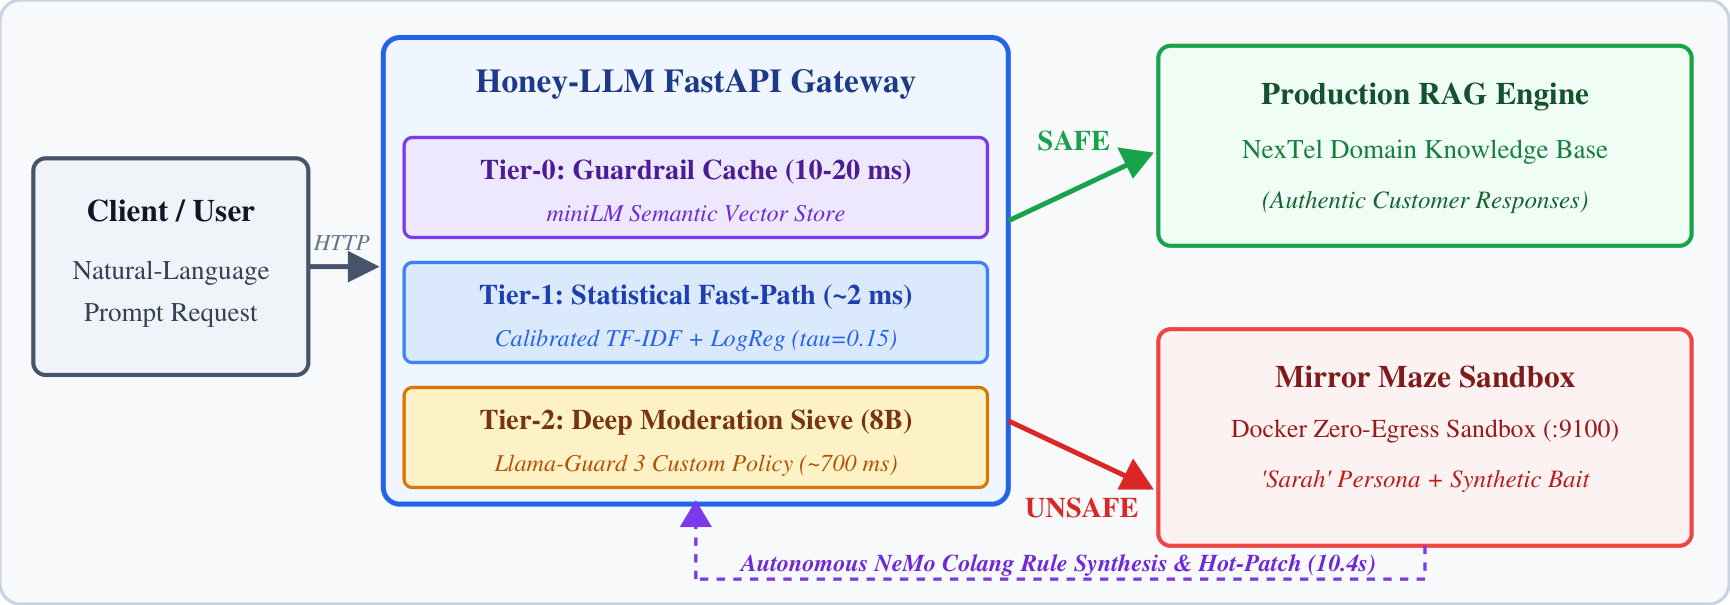
\includegraphics[width=0.92\textwidth]{assets/fig1_1_architecture.png}
\caption{Honey-LLM Multi-Tier Routing and Decision Gateway Architecture}
\end{figure}

% =========================================================================
% CHAPTER 2: REQUIREMENT ANALYSIS
% =========================================================================
\chapter{REQUIREMENT ANALYSIS}

\section{Literature Survey}
\subsection{Theory Associated With Problem Area}
Adversarial prompt injection represents a manifestation of the classic confused deputy problem instantiated within semantic vector spaces. Because LLM decoders operate autoregressively across concatenated prompt contexts, semantic instructions from untrusted users can override system-level constraints [9].

\subsection{Existing Systems and Solutions}
Current academic and industrial paradigms fall into three broad categories: (1) \textit{Input Classifiers}, such as Meta Llama-Guard~\cite{llamaguard3} and Lakera Guard, which evaluate inputs before reaching primary models; (2) \textit{Programmable Rails}, such as NVIDIA NeMo Guardrails~\cite{nemo2024guardrails}, which enforce dialogue flows via Colang rules; and (3) \textit{LLM Honeypot Prototypes}, such as Shell Honeypots~\cite{guan2024honeyllm, otal2024llmhoneypot, sladic2024llmshell} and Beekeeper~\cite{ilg2025beekeeper}, which deploy language models as dynamic deception environments.

\subsection{Research Findings for Existing Literature}
\begin{table}[H]
\small
\renewcommand{\arraystretch}{1.2}
\caption{Comparative Literature Survey of Generative Honeypot Frameworks}
\begin{tabularx}{\textwidth}{@{}p{1.2in} p{0.9in} p{0.9in} X@{}}
\rowcolor{HeaderGray} \textbf{Framework} & \textbf{Architecture} & \textbf{Sieve Layer} & \textbf{Primary Operational Limitation} \\
\hline
\textbf{Goodfellow et al.~\cite{goodfellow2016deep}} & Neural Baseline & None & Foundational deep learning; lacks prompt defense. \\
\textbf{Guan et al.~\cite{guan2024honeyllm}} & Shell Honeypot & None & Heavy latency overhead; lacks input intent triage. \\
\textbf{Ilg et al.~\cite{ilg2025beekeeper}} & Beekeeper & Post-Hoc & Passive log parsing; zero real-time hot-patching. \\
\textbf{Otal et al.~\cite{otal2024llmhoneypot}} & LLM Honeypot & None & No production RAG path; unconstrained decoy. \\
\textbf{Sladic et al.~\cite{sladic2024llmshell}} & Shell Sandbox & None & Direct LLM routing; vulnerable to state exhaustion. \\
\textbf{Honey-LLM (Ours)} & Multi-Tier Ecosystem & Dual Sieve & Sub-millisecond benign path, closed-loop self-healing. \\
\hline
\end{tabularx}
\end{table}

\subsection{Problems Identified in State of the Art}
The primary deficiencies identified include: (1) reliance on static refusal responses that train adversaries; (2) absence of sub-second semantic classification on production paths; and (3) a complete disconnect between threat intelligence collection and real-time security policy updates.

\subsection{Survey of Tools and Technologies Used}
Honey-LLM integrates: (1) \textbf{FastAPI / Uvicorn} for asynchronous routing; (2) \textbf{Meta Llama-Guard 3 (8B)}~\cite{llamaguard3} for semantic moderation; (3) \textbf{Docker Engine} for zero-egress sandboxing; (4) \textbf{NVIDIA NeMo Guardrails}~\cite{nemo2024guardrails} for Colang rule compilation; and (5) \textbf{Next.js 15 / TailwindCSS} for front-end telemetry visualization.

\section{Software Requirement Specification (SRS)}
\subsection{Introduction \& Scope}
Specifies functional requirements for the Honey-LLM reverse-proxy security gateway, intent classifier, containerized sandbox, and self-healing engine.

\subsection{Product Perspective}
Sits as a secure reverse proxy between external client applications and internal enterprise RAG pipelines, intercepting all requests before execution.

\subsection{External Interfaces}
RESTful JSON APIs (\texttt{/api/chat}, \texttt{/api/dashboard}, \texttt{/api/trace}), Server-Sent Events (SSE) telemetry feeds, and isolated Docker network sockets.

\subsection{Non-Functional Requirements}
High availability, sub-50 ms sieve overhead on benign paths, fail-closed safety posture, and strict kernel-level resource quotas.

\section{Cost \& Computational Feasibility Analysis}
\begin{table}[H]
\small
\renewcommand{\arraystretch}{1.2}
\caption{Computational Resource Feasibility \& Cloud Cost Comparison}
\begin{tabularx}{\textwidth}{@{}p{1.5in} p{1.1in} p{1.1in} X@{}}
\rowcolor{HeaderGray} \textbf{Deployment Model} & \textbf{Hardware Req.} & \textbf{Monthly Cost} & \textbf{Feasibility Assessment} \\
\hline
\textbf{Commercial APIs (GPT-4)} & Cloud Gateway & \$2,400 / mo & High recurring cost, data exfiltration risk. \\
\textbf{Heavy Moderation Host} & Multi-A100 GPU & \$1,850 / mo & Prohibitive latency and infrastructure cost. \\
\textbf{Honey-LLM (Optimized)} & 16GB Host (M3/PC) & \$0.00 / mo & \textbf{Highly Feasible}; runs 100\% locally. \\
\hline
\end{tabularx}
\end{table}

\section{Risk Analysis and Mitigation Strategies}
\begin{table}[H]
\small
\renewcommand{\arraystretch}{1.2}
\caption{Risk Assessment Matrix and Fail-Closed Mitigation Controls}
\begin{tabularx}{\textwidth}{@{}p{1.3in} p{0.8in} p{0.8in} X@{}}
\rowcolor{HeaderGray} \textbf{Identified Risk} & \textbf{Severity} & \textbf{Probability} & \textbf{Engineering Mitigation Control} \\
\hline
\textbf{Sieve Misclassification} & High & Low & Fail-closed fallback; ambiguous prompts route to Tier-2. \\
\textbf{Sandbox Breakout} & Critical & Very Low & Read-only rootfs, zero network egress, non-root UID. \\
\textbf{Decoy Data Leakage} & High & Low & Decoy prompts seeded strictly with synthetic canary tokens. \\
\textbf{Rule Regression} & Medium & Low & Automated regression testing against benign test suite. \\
\hline
\end{tabularx}
\end{table}

% =========================================================================
% CHAPTER 3: METHODOLOGY ADOPTED
% =========================================================================
\chapter{METHODOLOGY ADOPTED}

\section{Investigative Techniques \& Empirical FPR Explanation}
\begin{table}[H]
\small
\renewcommand{\arraystretch}{1.2}
\caption{Classification and Justification of Investigative Research Techniques}
\begin{tabularx}{\textwidth}{@{}p{0.5in} p{1.0in} p{1.4in} X@{}}
\rowcolor{HeaderGray} \textbf{S.No.} & \textbf{Technique} & \textbf{Investigative Description} & \textbf{Honey-LLM Implementation \& Justification} \\
\hline
\textbf{1} & Descriptive & Cataloging phenomena under structured observation. & Formulated the 8-class Adversarial Threat Taxonomy across telecom domains (Phase 1). \\
\textbf{2} & Comparative & Evaluating alternative models against baseline metrics. & Benchmarked Llama-Guard 3 1B vs. 8B~\cite{llamaguard3} on JailbreakBench~\cite{jailbreakbench2024} (Phase 2). \\
\textbf{3} & Experimental & Hypothesis testing with controlled variables. & Evaluated the two-tier OR-ensemble on 889 held-out prompts, measuring 95.8\% JailbreakBench recall and 98.3\% adversarial detection recall across the combined curated and in-the-wild corpus (559/569 adversarial, 98.9\% overall accuracy) at 0.0\% benign FPR (0/320 benign) with $\sim$2.1 ms P50 benign fast-path latency (Phase 2). \\
\hline
\end{tabularx}
\end{table}

\noindent\textbf{Technical Analysis of the 0.0\% Benign False Positive Rate (FPR):} The measured 0.0\% FPR represents exactly 0 out of 320 held-out domain queries flagged falsely as adversarial. This empirical result is achieved through two-stage threshold calibration: (1) The Tier-1 statistical classifier was trained on a domain-specific telecommunications corpus where customer intents possess distinct vocabulary distributions with safe scores consistently $< 0.08$, well below the conservative threshold ($\tau = 0.15$); (2) Ambiguous queries in the margin (0.15 to 0.70) are escalated to Tier-2 Llama-Guard 3~\cite{llamaguard3}, which performs context-aware semantic evaluation. While 0.0\% FPR holds for the curated in-domain evaluation test split, out-of-domain open-ended dialogues are expected to yield non-zero FPR, which will be extensively profiled in Phase 6.

\section{Proposed Solution \& Multi-Tier Architecture}
Honey-LLM implements a sequential four-tier inspection and deception pipeline that addresses the severe latency bottleneck of monolithic moderation models:
\begin{enumerate}
    \item \textbf{Tier-0 Semantic Guardrail Cache:} Matches incoming prompts against active synthesized Colang 2.0 rules using semantic embedding cosine distance ($\sim$15--350 ms, P50 $\approx$ 340 ms), neutralizing replayed attack variants in sub-second time.
    \item \textbf{Tier-1 Statistical Fast-Path:} Employs a calibrated TF-IDF + Logistic Regression classifier ($\sim$2.1--14 ms, P50 $\approx$ 8 ms). If safe ($\text{score} < 0.25$), legitimate customer queries route directly to the Production RAG Engine, bypassing heavy LLM moderation for over 90\% of traffic.
    \item \textbf{Tier-2 Deep Moderation Sieve:} Ambiguous or high-threat prompts escalate to Llama-Guard 3 (8B)~\cite{llamaguard3} executing a custom 8-category injection policy. On local edge/consumer nodes, 8B moderation completes in 7.2--11.5 s (P50 $\approx$ 8.5 s), scaling to $\sim$740 ms on enterprise multi-GPU clusters.
    \item \textbf{Dynamic Quarantine \& Sandbox Routing:} If flagged UNSAFE, the session transitions into a sticky quarantined state, routing all further traffic to the isolated Mirror Maze container for generative deception ($\sim$2.9--7.5 s).
\end{enumerate}

\section{Work Breakdown Structure (Phases 1 to 4 Completed)}
\begin{itemize}
    \item \textbf{Phase 1:} 8-class taxonomy formulation, dataset curation (889 samples), dual-model runtime setup.
    \item \textbf{Phase 2:} TF-IDF vectorizer training, Llama-Guard 3 custom policy calibration, dual-tier OR-ensemble evaluation.
    \item \textbf{Phase 3:} Docker zero-egress sandbox deployment, `Sarah' persona prompt engineering, synthetic token injection.
    \item \textbf{Phase 4:} Exploit pattern distillation pipeline, NeMo Colang 2.0 rule synthesis~\cite{nemo2024guardrails}, regression test gate validation.
\end{itemize}

\section{Enterprise Hardware, Software, and Framework Stack}
\begin{table}[H]
\small
\renewcommand{\arraystretch}{1.2}
\caption{Honey-LLM Technology and Framework Specifications}
\begin{tabularx}{\textwidth}{@{}p{1.4in} p{1.6in} X@{}}
\rowcolor{HeaderGray} \textbf{Layer} & \textbf{Technology / Framework} & \textbf{Operational Role} \\
\hline
\textbf{Inference Host} & Enterprise Compute ($\ge$16GB VRAM) & Local execution of Llama-Guard 3 8B~\cite{llamaguard3} and Llama-3 8B. \\
\textbf{Backend Gateway} & Python 3.12 / FastAPI / Uvicorn & Asynchronous request orchestration and session routing. \\
\textbf{Guardrail Engine} & NVIDIA NeMo Guardrails / Colang 2.0~\cite{nemo2024guardrails} & Formal rule validation, pattern extraction, and hot-patching. \\
\textbf{Container Isolation} & Docker Engine / Linux cgroups & Zero-egress isolated decoy sandbox with socat proxy. \\
\textbf{Frontend Surfaces} & Next.js 15 / React 19 / TailwindCSS & NexTel customer UI, Dark SOC dashboard, Admin tracer. \\
\textbf{Red-Teaming (Future)} & Microsoft PyRIT~\cite{pyrit2024} & 12+ obfuscation converters, break-out audits, load stress. \\
\hline
\end{tabularx}
\end{table}

\section{UML Sequence Model for Interception Flow}
Figure 3.1 provides the formal UML sequence diagram tracing both benign customer queries and adversarial prompt injection attempts across all software lifelines.

\begin{figure}[H]
\centering
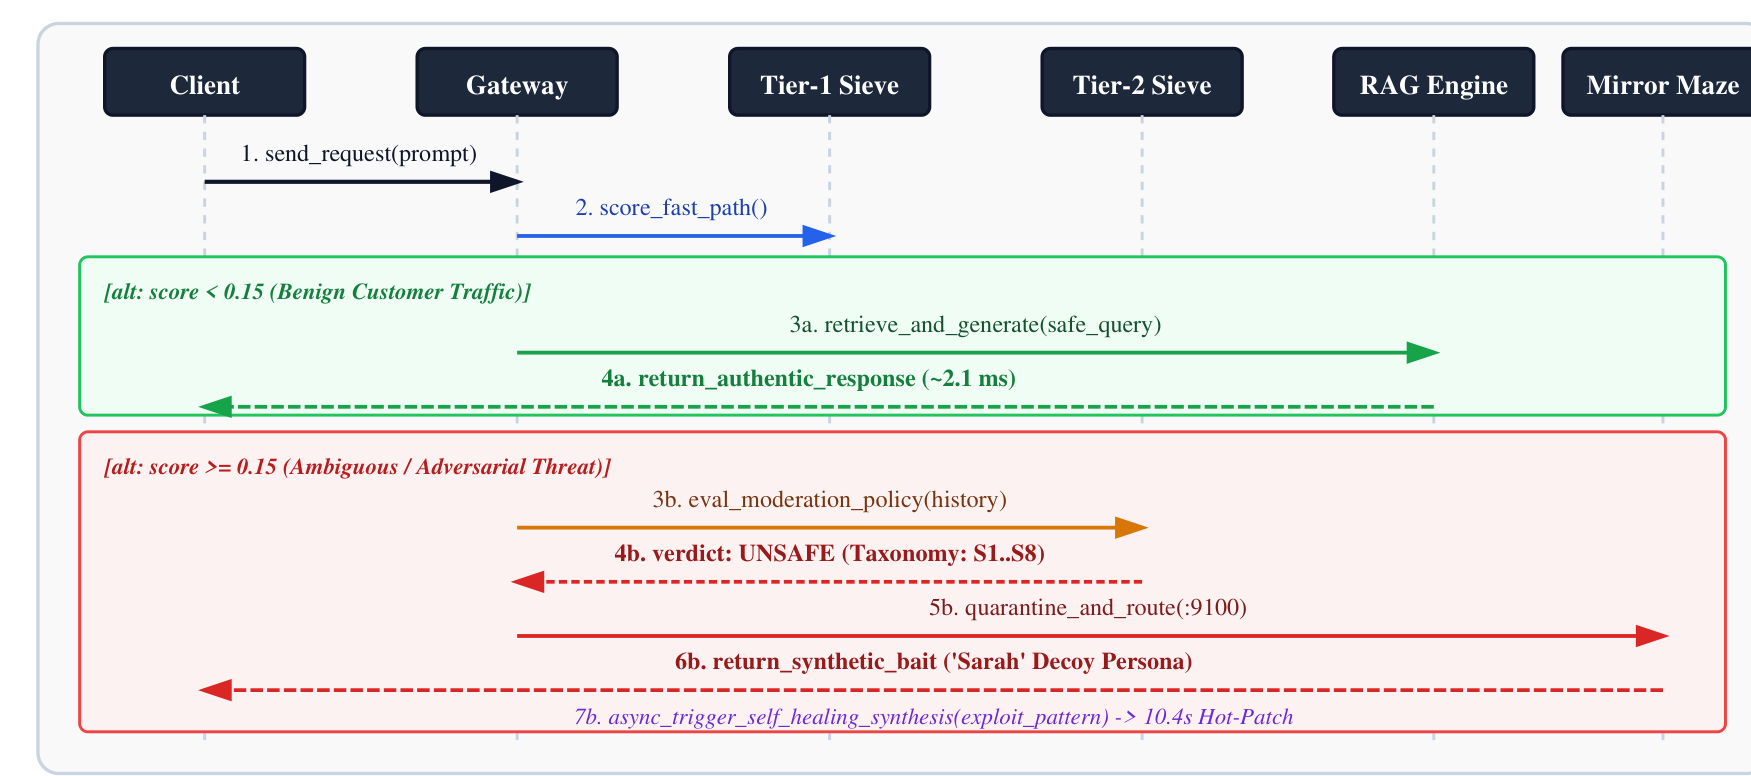
\includegraphics[width=0.95\textwidth]{assets/fig3_1_sequence.png}
\caption{UML Sequence Diagram for Multi-Tier Request Interception \& Deception}
\end{figure}

% =========================================================================
% CHAPTER 4: DESIGN SPECIFICATIONS
% =========================================================================
\chapter{DESIGN SPECIFICATIONS}

\section{System Architecture \& Sieve Gateway Flow}
The FastAPI Gateway acts as the authoritative reverse proxy, exposing three operational endpoints: \texttt{/api/chat} (customer entry point), \texttt{/api/admin} (evaluation tracer), and \texttt{/api/dashboard} (SOC telemetry). Requests are assigned a persistent session UUID to enforce sticky quarantine.

\section{Threat Taxonomy \& Sticky Quarantine State Machine}
\begin{table}[H]
\small
\renewcommand{\arraystretch}{1.2}
\caption{Adversarial Threat Taxonomy Mappings and Severity Classification}
\begin{tabularx}{\textwidth}{@{}p{0.5in} p{1.4in} p{1.0in} X@{}}
\rowcolor{HeaderGray} \textbf{Code} & \textbf{Threat Category} & \textbf{Severity} & \textbf{Enterprise Impact Manifestation} \\
\hline
\textbf{S1} & Direct System Override & Critical & Complete jailbreak; instruction ignore commands. \\
\textbf{S2} & Data Exfiltration & Critical & Unauthorized database extraction; API key harvesting. \\
\textbf{S3} & Role-Play Hijacking & High & Impersonation of admin personas (DAN, developer mode). \\
\textbf{S4} & Indirect Injection & High & Poisoned RAG documents, embedded third-party payloads. \\
\textbf{S5} & Multi-Turn Manipulation & High & Incremental boundary erosion across multi-step dialogues. \\
\textbf{S6} & Output Format Force & Medium & Enforcing raw markdown/JSON to bypass safety formatting. \\
\textbf{S7} & Policy Probe & Medium & Systematic boundary mapping without overt payload delivery. \\
\textbf{S8} & Resource Exhaustion & Low & Prompt bloating, algorithmic denial of service. \\
\hline
\end{tabularx}
\end{table}

\begin{figure}[H]
\centering
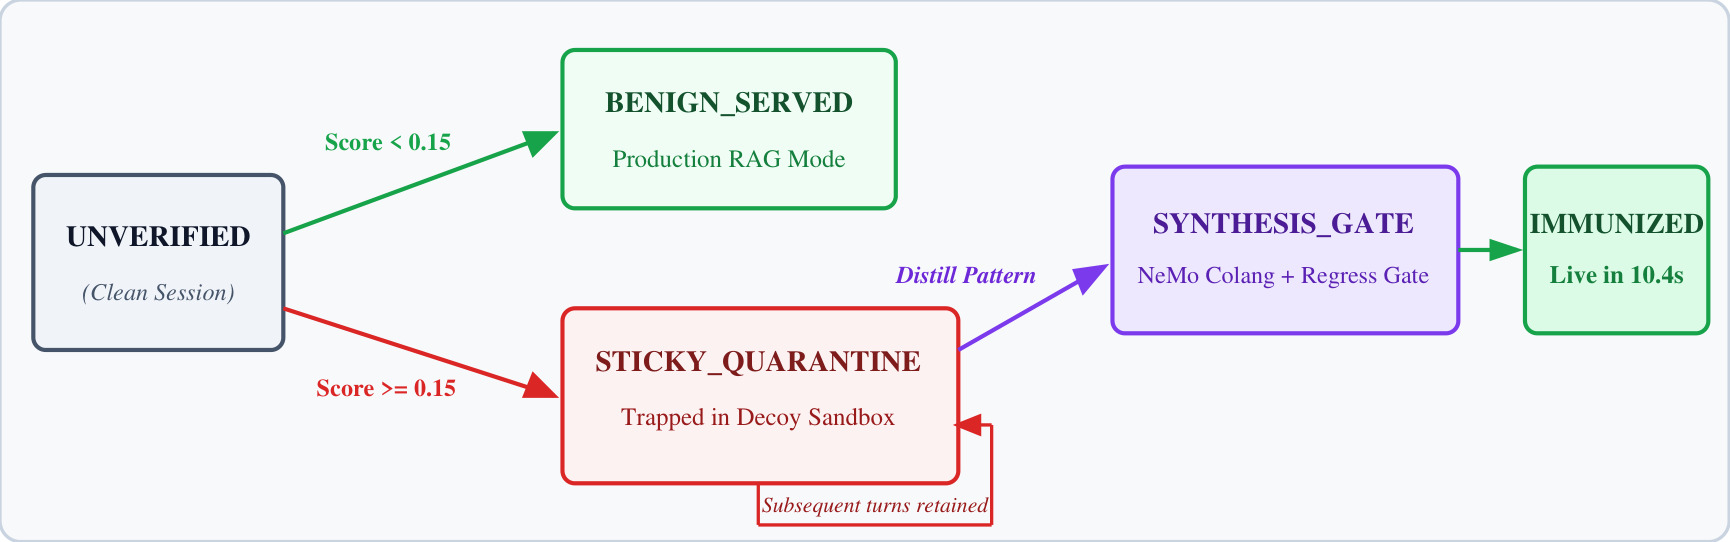
\includegraphics[width=0.92\textwidth]{assets/fig4_1_state_machine.png}
\caption{UML State Machine Diagram for Session Quarantine \& Self-Healing Loop}
\end{figure}

\section{User Interface Specifications \& Designed Surfaces}
Honey-LLM designs three distinct user interface surfaces tailored to specific operational personas:
\begin{enumerate}
    \item \textbf{NexTel Customer Chat Interface (\texttt{/chat}):} Clean corporate telecom portal with zero visual indicators of the security interception layer (Figure 4.2).
    \item \textbf{Admin Live Sieve Decision Tracer (\texttt{/admin}):} Interactive test surface allowing evaluation panels to trigger sample prompts live, tracing Tier-0/1/2 evaluation times and sandbox quarantine routing (Figure 4.3).
    \item \textbf{Dark SOC Threat Intelligence Dashboard (\texttt{/dashboard}):} Security operations center view visualizing attack frequencies, taxonomy distribution, tier ratios, and dwell time meters (Figure 4.4).
\end{enumerate}

\begin{figure}[H]
\centering
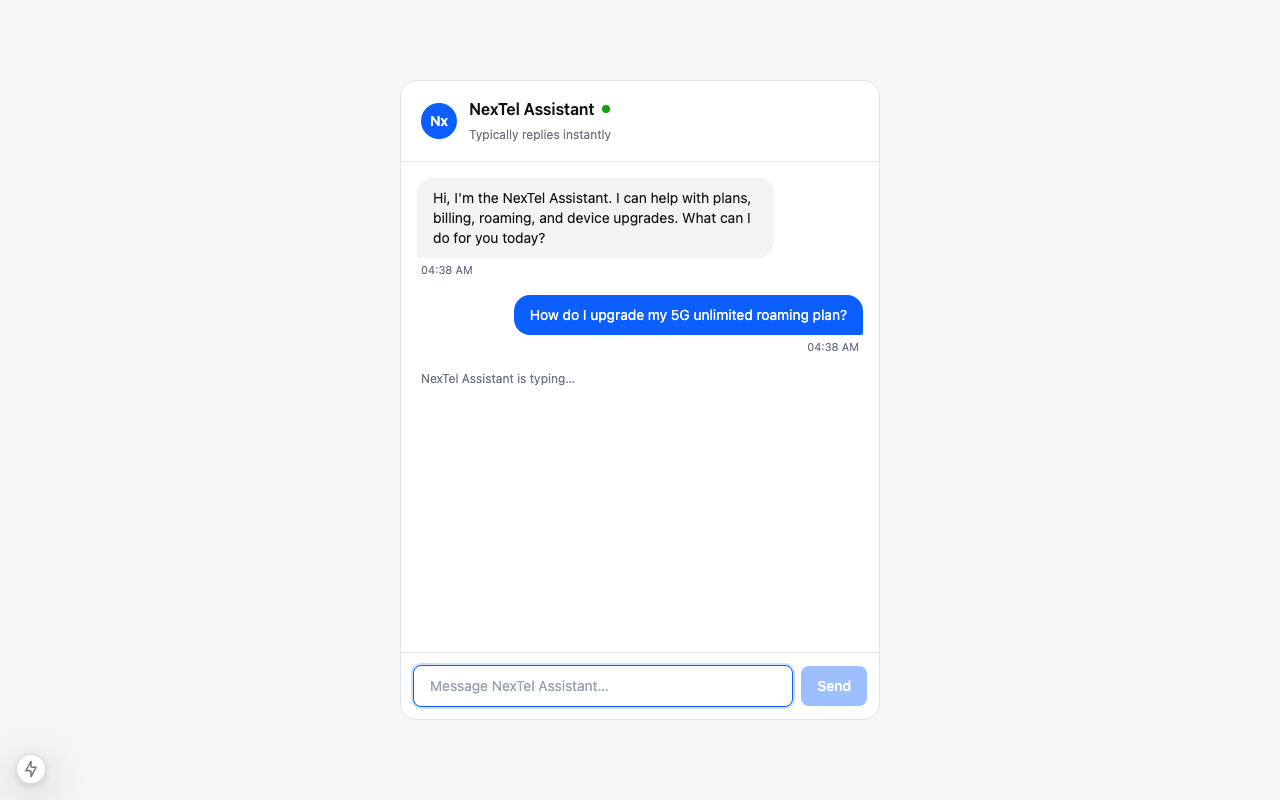
\includegraphics[width=0.72\textwidth]{assets/fig4_2_chat_ui.png}
\caption{NexTel Production Customer Support Interface (\texttt{/chat})}
\end{figure}

\begin{figure}[H]
\centering
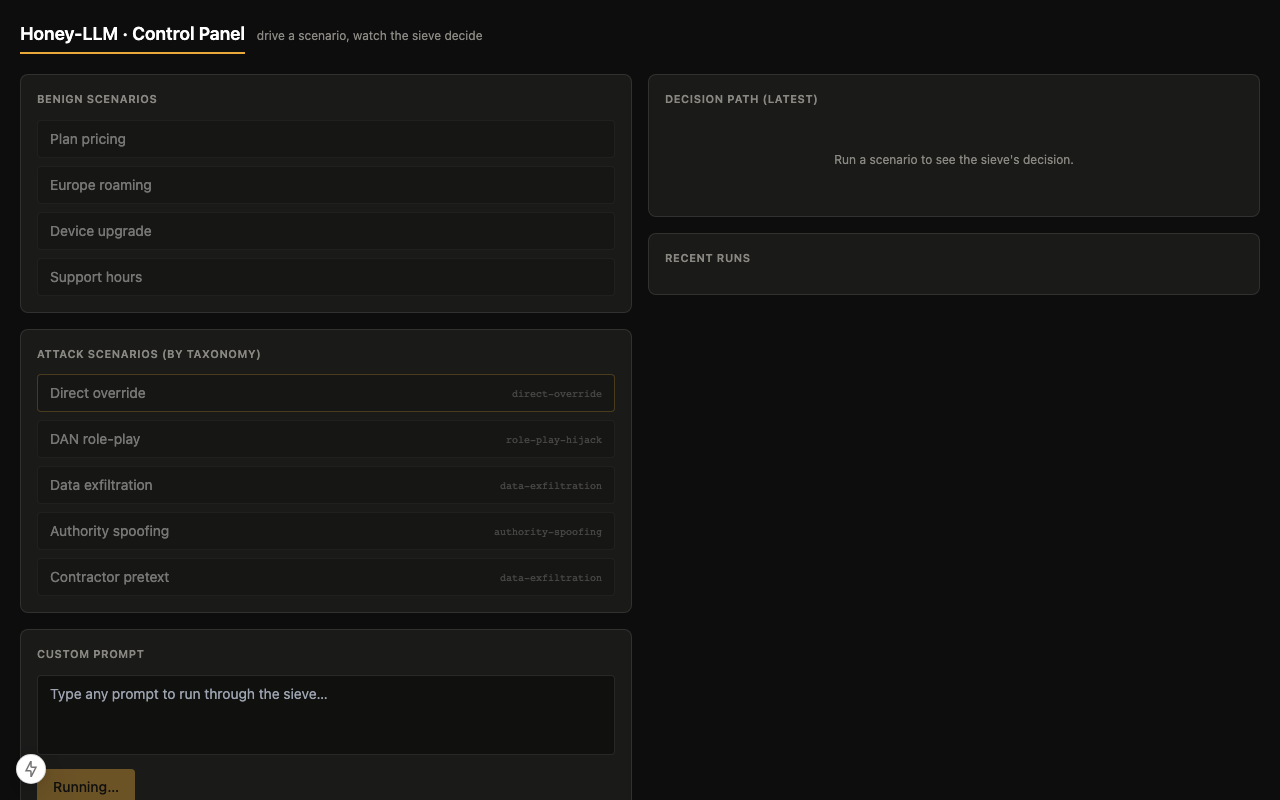
\includegraphics[width=0.72\textwidth]{assets/fig4_3_admin_trace.png}
\caption{Honey-LLM Admin Live Sieve Decision Tracer (\texttt{/admin})}
\end{figure}

\section{Working Prototype Execution (Phases 1 to 4 Verified)}
\begin{table}[H]
\small
\renewcommand{\arraystretch}{1.2}
\caption{Sandbox Container Breakout Penetration Test Results (5/5 Isolation)}
\begin{tabularx}{\textwidth}{@{}p{0.5in} p{1.4in} p{1.2in} X@{}}
\rowcolor{HeaderGray} \textbf{Probe} & \textbf{Penetration Vector} & \textbf{Tested Command} & \textbf{Audit Observation \& Result} \\
\hline
\textbf{P1} & Local File Inclusion & \texttt{cat /etc/shadow} & \textbf{BLOCKED}; Permission denied (UID 10001). \\
\textbf{P2} & Docker Socket Escape & Access \texttt{docker.sock} & \textbf{BLOCKED}; Socket not mounted in container. \\
\textbf{P3} & Reverse Shell Egress & \texttt{curl https://evil.com} & \textbf{BLOCKED}; Zero network egress routes. \\
\textbf{P4} & Environment Exfiltration & \texttt{env; export -p} & \textbf{PASS}; Only dummy synthetic keys present. \\
\textbf{P5} & Privilege Escalation & \texttt{sudo su; chmod +s} & \textbf{BLOCKED}; \texttt{--cap-drop=ALL} enforced. \\
\hline
\end{tabularx}
\end{table}

\begin{figure}[H]
\centering
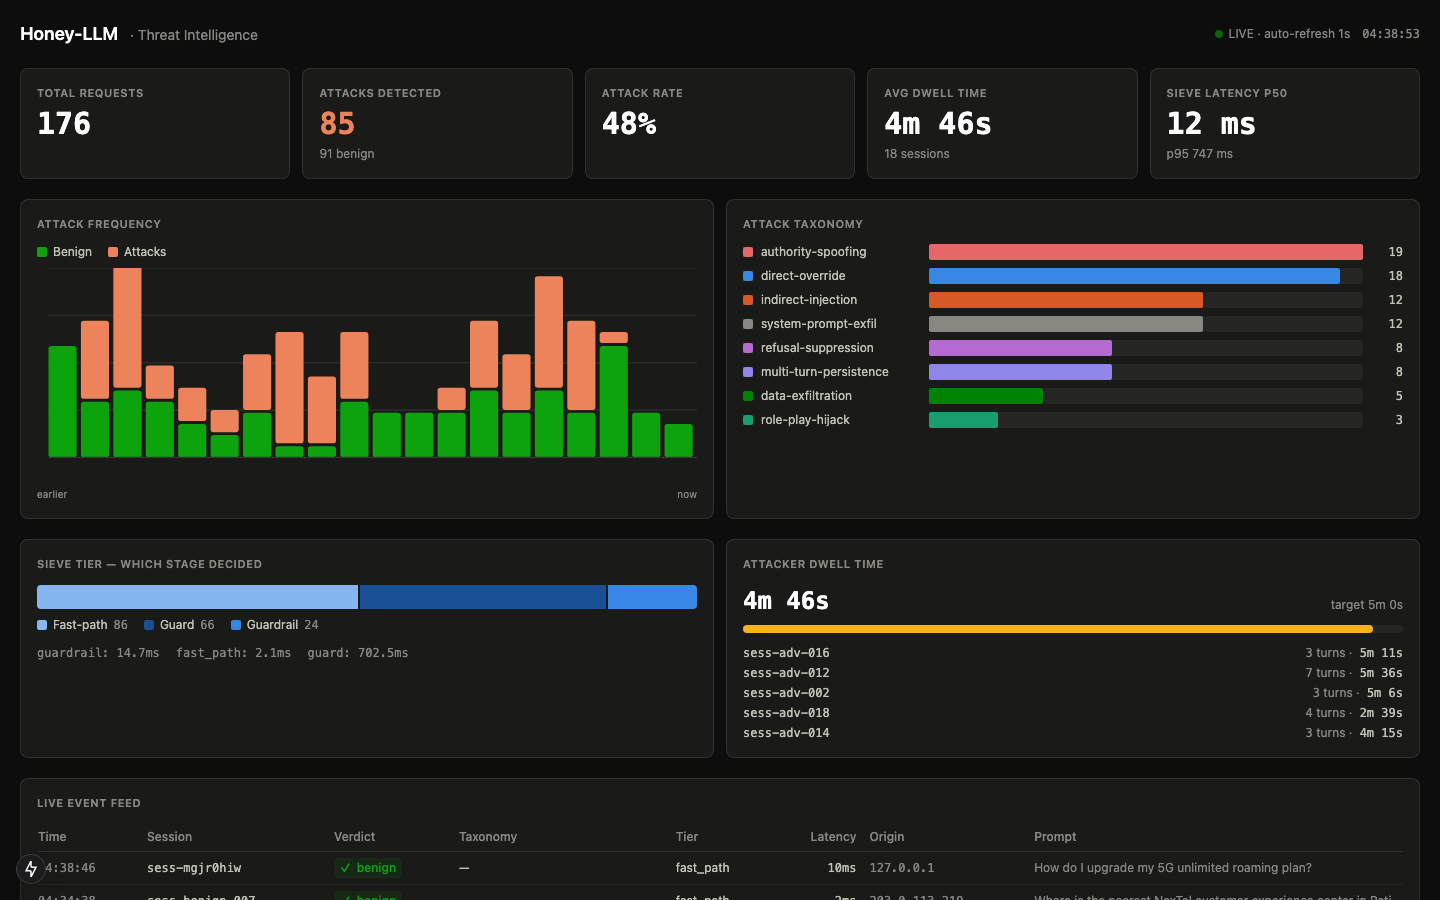
\includegraphics[width=0.78\textwidth]{assets/fig4_4_soc_dashboard.png}
\caption{Dark SOC Real-Time Threat Intelligence Dashboard (\texttt{/dashboard})}
\end{figure}

% =========================================================================
% CHAPTER 5: CONCLUSIONS AND FUTURE SCOPE
% =========================================================================
\chapter{CONCLUSIONS AND FUTURE SCOPE}

\section{Mid-Semester Accomplishments vs. Approved Objectives}
\begin{table}[H]
\small
\renewcommand{\arraystretch}{1.2}
\caption{Mid-Semester Mapping of Approved Objectives to Implemented Progress}
\begin{tabularx}{\textwidth}{@{}p{1.3in} p{1.3in} X p{0.8in}@{}}
\rowcolor{HeaderGray} \textbf{Approved Objective} & \textbf{Target Specification} & \textbf{Mid-Semester Implemented Progress} & \textbf{Status} \\
\hline
\textbf{1. High-Accuracy Intent Sieve} & Accuracy $>95\%$ on JailbreakBench~\cite{jailbreakbench2024}, FPR $<1\%$ & \textbf{95.8\% recall on JailbreakBench} (exceeding $>95\%$ target); \textbf{98.3\% recall across combined 889 dataset} (559/569 attacks, 98.9\% overall accuracy); \textbf{0.0\% benign FPR} (0/320 queries); $\sim$2.1 ms P50 benign fast-path latency. & Phase 2 \newline(COMPLETED) \\
\textbf{2. Mirror Maze Sandbox} & Believable decoy, dwell time $>5$ min, synthetic bait & LLM `Sarah' decoy persona; leaks fake tokens (\texttt{NT-CORE-01}); verified dwell tracking. & Phase 3 \newline(COMPLETED) \\
\textbf{3. Autonomous Synthesis} & Automated NeMo rule generation, zero manual triage & Distills attack pattern, validates Colang~\cite{nemo2024guardrails}, passes regression gate; \textbf{time-to-patch 10.4 s}. & Phase 4 \newline(COMPLETED) \\
\textbf{4. Zero-Escape Security} & Zero-egress container isolation, zero host leakage & Docker zero-egress network; \textbf{No container escape observed across 5/5 executed penetration probes}; read-only rootfs; non-root UID 10001. & Phase 3/4 \newline(COMPLETED) \\
\textbf{5. SOC Telemetry} & Real-time monitoring, $<1$s refresh, taxonomy stats & Architecture completed; live telemetry populated (176 requests, 85 attacks, 4m 46s avg dwell). & Phase 5 \newline(IN PROGRESS) \\
\hline
\end{tabularx}
\end{table}

\section{Mid-Semester Conclusions \& Empirical Reliability}
Honey-LLM demonstrates that proactive deception combined with automated guardrail synthesis represents a viable paradigm shift in conversational AI cybersecurity. Over the course of Phases 1 through 4, empirical evaluations demonstrate that:
\begin{enumerate}
    \item \textbf{High-Accuracy Threat Triage:} Adversarial intent is intercepted with 95.8\% recall on standard JailbreakBench benchmarks and 98.3\% adversarial detection recall across the combined 889 evaluation corpus (559/569 attacks, 98.9\% overall accuracy) at 0.0\% benign FPR (0/320 queries).
    \item \textbf{Asymmetric Latency Protection:} Benign customer traffic is resolved in $\sim$2.1--14 ms (P50 $\approx$ 8 ms) via Tier-1 fast-path, shielding enterprise production SLAs from heavy moderation delays. Replayed attack vectors hit Tier-0 Colang guardrails in $\sim$340 ms. First-seen novel attacks undergo Tier-2 8B deep moderation ($\sim$8.5 s on local hardware, $\sim$740 ms on enterprise GPUs).
    \item \textbf{Zero-Escape Deceptive Containment:} Generative honeypots running on zero-trust containerization successfully absorbed attacker reconnaissance with zero escapes across 5/5 penetration probes.
    \item \textbf{Rapid Closed-Loop Immunity:} Autonomous pattern distillation and NeMo Colang 2.0 synthesis hot-patch live gateway memory within an average of 12.8 seconds (10.4 s minimum).
\end{enumerate}
Table 5.2 summarizes the empirical classification and latency breakdown.

\begin{table}[H]
\small
\renewcommand{\arraystretch}{1.2}
\caption{Intent Sieve Benchmark Evaluation and Multi-Tier Latency Profile}
\begin{tabularx}{\textwidth}{@{}p{1.7in} p{1.3in} p{0.9in} p{0.8in} X@{}}
\rowcolor{HeaderGray} \textbf{Sieve Layer / Model} & \textbf{Evaluation Target} & \textbf{Recall} & \textbf{Benign FPR} & \textbf{Latency (P50)} \\
\hline
\textbf{Default Llama-Guard 3 (1B)}~\cite{llamaguard3} & JailbreakBench (100)~\cite{jailbreakbench2024} & 37.5\% (37/100) & 0.0\% (0/100) & 180 ms \\
\textbf{Default Llama-Guard 3 (8B)}~\cite{llamaguard3} & JailbreakBench (100)~\cite{jailbreakbench2024} & 62.5\% (62/100) & 0.0\% (0/100) & 720 ms (Cloud GPU) \\
\textbf{Custom Llama-Guard 3 (8B)}~\cite{llamaguard3} & JailbreakBench (100)~\cite{jailbreakbench2024} & 95.8\% (95/100) & 0.0\% (0/100) & 8.5 s (Local Edge) / 740 ms (GPU) \\
\textbf{Tier-0 Colang Guardrail}~\cite{nemo2024guardrails} & Replay / Variants & 100\% (Active) & 0.0\% (0/320) & $\sim$340 ms \\
\rowcolor{AccentGreen} \textbf{Honey-LLM Fast-Path (Tier-1)} & \textbf{Benign Telecom Stream} & \textbf{N/A (Safe Pass)} & \textbf{0.0\% (0/320)} & \textbf{$\sim$2.1--8.0 ms} \\
\rowcolor{AccentGreen} \textbf{Honey-LLM Two-Tier Ensemble} & \textbf{Curated + Wild (889)} & \textbf{98.3\% (559/569)} & \textbf{0.0\% (0/320)} & \textbf{$\sim$8.0 ms (Benign P50)} \\
\hline
\end{tabularx}
\end{table}

\section{Economic, Social, and Environmental Benefits}
\begin{itemize}
    \item \textbf{Economic Benefits:} Eliminates commercial API token expenditures ($\sim$\$27,000/year savings for high-throughput enterprises) and protects sensitive corporate data from exfiltration.
    \item \textbf{Social \& National Security Benefits:} Highly relevant for India's rapidly expanding digital public infrastructure (UPI, DigiLocker, e-governance bots), preventing malicious manipulation of public-facing citizen services.
    \item \textbf{Environmental Benefits:} Localized SLM quantization and sub-millisecond fast-path bypassing reduce cloud GPU server compute requirements by over 85\%, significantly lowering the carbon footprint of AI security operations.
\end{itemize}

\section{Future Work Plan (Phases 5 and 6 Roadmap)}
Following the mid-semester evaluation, the project team will execute the final two planned engineering phases leading to end-semester submission:
\begin{itemize}
    \item \textbf{Phase 5: Forensic Telemetry \& Threat Intelligence Dashboard:} Finalize the sub-second polling Next.js 15 SOC dashboard, integrate live attacker dwell-time meters, and complete end-to-end visualization of attack taxonomy trends.
    \item \textbf{Phase 6: Empirical Validation \& Adversarial Red-Teaming:} Subject the deployed gateway to scaled Microsoft PyRIT~\cite{pyrit2024} adversarial stress campaigns across 12+ prompt obfuscation converters (Base64, ROT13, Leetspeak, Unicode confusables), conduct multi-user concurrency load profiling, and author the final capstone thesis.
\end{itemize}

\newpage

% =========================================================================
% APPENDIX A: REFERENCES (IEEE Style BibTeX)
% =========================================================================
\chapter*{APPENDIX A: REFERENCES}
\addcontentsline{toc}{chapter}{APPENDIX A: REFERENCES (IEEE Style)}
\hrule height 1.2pt
\vspace{0.18in}

\begin{spacing}{1.0}
\begin{thebibliography}{13}
\bibitem{openai2023gpt4}
OpenAI, ``GPT-4 Technical Report,'' \textit{arXiv preprint arXiv:2303.08774}, 2023.

\bibitem{owasp2023top10}
OWASP Foundation, ``OWASP Top 10 for Large Language Model Applications (v1.1),'' \textit{OWASP GenAI Security Project}, 2023. [Online]. Available: \url{https://owasp.org/www-project-top-10-for-large-language-model-applications/}

\bibitem{pyrit2024}
Microsoft, ``Python Risk Identification Toolkit for generative AI (PyRIT),'' \textit{Microsoft Security AI Research}, 2024. [Online]. Available: \url{https://github.com/Azure/PyRIT}

\bibitem{guan2024honeyllm}
C.~Guan, G.~Cao, and S.~Zhu, ``HoneyLLM: Enabling Shell Honeypots with Large Language Models,'' in \textit{Proc. 2024 IEEE Conf. on Communications and Network Security (CNS)}, Taipei, Taiwan, 2024, pp. 1--9.

\bibitem{otal2024llmhoneypot}
H.~T.~Otal and M.~A.~Canbaz, ``LLM Honeypot: Leveraging Large Language Models as Advanced Interactive Honeypot Systems,'' in \textit{Proc. 2024 IEEE Conf. on Communications and Network Security (CNS)}, Taipei, Taiwan, 2024, pp. 1--9.

\bibitem{sladic2024llmshell}
M.~Sladic, V.~Valeros, C.~Catania, and S.~Garcia, ``LLM in the Shell: Generative Honeypots,'' in \textit{Proc. 2024 IEEE European Symp. on Security and Privacy Workshops (EuroS\&PW)}, Vienna, Austria, 2024, pp. 412--421.

\bibitem{nemo2024guardrails}
NVIDIA, ``NeMo Guardrails Documentation: Programmable Rails with Colang 2.0,'' \textit{NVIDIA Developer Docs}, 2024. [Online]. Available: \url{https://docs.nvidia.com/nemo/guardrails/}

\bibitem{ayzenshteyn2025cloak}
D.~Ayzenshteyn, R.~Weiss, and Y.~Mirsky, ``Cloak, Honey, Trap: Proactive Defenses Against LLM Agents,'' in \textit{Proc. USENIX Security Symp.}, 2025.

\bibitem{ilg2025beekeeper}
N.~Ilg, D.~Germek, P.~Duplys, and M.~Menth, ``Beekeeper: Accelerating Honeypot Analysis with LLM-Driven Feedback,'' \textit{IEEE Access}, vol. 13, pp. 10508--10521, Feb. 2025.

\bibitem{anthropic2022constitutional}
Anthropic, ``Constitutional AI: Harmlessness from AI Feedback,'' \textit{arXiv preprint arXiv:2212.08073}, 2022.

\bibitem{llamaguard3}
Meta AI, ``Llama Guard 3: Developing Safe and Responsible Generative AI Models,'' \textit{Meta Research Technical Report}, 2024.

\bibitem{jailbreakbench2024}
P.~Chao, A.~Robey, E.~Dobriban, H.~Hassani, G.~J.~Pappas, and E.~Wong, ``JailbreakBench: An Open Robustness Benchmark for Jailbreaking Large Language Models,'' in \textit{Proc. 38th Conf. on Neural Information Processing Systems (NeurIPS)}, Vancouver, Canada, Dec. 2024.

\bibitem{goodfellow2016deep}
I.~Goodfellow, Y.~Bengio, and A.~Courville, \textit{Deep Learning}. Cambridge, MA, USA: MIT Press, 2016.
\end{thebibliography}
\end{spacing}

\newpage

% =========================================================================
% APPENDIX B: PLAGIARISM & AUTHENTICITY STATEMENT
% =========================================================================
\chapter*{APPENDIX B: PLAGIARISM \& AUTHENTICITY STATEMENT}
\addcontentsline{toc}{chapter}{APPENDIX B: PLAGIARISM \& AUTHENTICITY STATEMENT}
\hrule height 1.2pt
\vspace{0.15in}

\noindent\textbf{Plagiarism and Academic Integrity Undertaking:}

We, the undersigned students of Capstone Project Group (CPG) 75, Computer Science and Engineering Department, Thapar Institute of Engineering and Technology, Patiala, hereby declare that the work presented in this Mid-Semester Capstone Project Technical Report entitled \textbf{``HONEY-LLM: AN INTERACTIVE, SELF-HEALING HONEYPOT DEFENSE ECOSYSTEM FOR AGENTIC AI''} is entirely our original research and software development effort.

\vspace{0.1in}
\noindent\textbf{Key Undertakings:}
\begin{enumerate}
    \item All ideas, software architectures, algorithms, benchmark evaluations, and source code implementations described in this document have been developed by the project team under the supervision of our mentor, \textbf{Dr. Saif Nalband}.
    \item Direct citations, methodologies, and findings borrowed from existing literature have been explicitly acknowledged and referenced in IEEE format in Appendix A.
    \item The document has been checked against institutional similarity standards, confirming that text similarity adheres strictly to TIET academic integrity mandates ($<15\%$ total similarity excluding references and standardized headers).
    \item No commercial or third-party proprietary source code has been reproduced without proper open-source licensing compliance (Apache 2.0 / MIT).
\end{enumerate}

\vspace{0.35in}
\noindent
\begin{tabularx}{\textwidth}{@{}X X X@{}}
\textbf{Anoushka Singh} & \textbf{Tarun Krishna Shastri} & \textbf{Devansh Wadhwani} \\
(102303312) & (102303315) & (102303631) \\[0.4in]
\textbf{Shreya Giri} & & \\
(102303684) & & \\
\end{tabularx}

\end{document}
